\usetikzlibrary{bending}
\begin{tikzpicture}[
  imgnode/.style={inner sep=0pt, draw=black!35, line width=1.0pt},
  titletext/.style={font=\bfseries},
  captiontext/.style={font=\small\itshape, align=center, text width=6.0cm},
  >={Latex[length=2mm,width=1.4mm,bend]},
  actionarr/.style={->, very thick, steelblue31119180!70!black},
  actionlabel/.style={font=\scriptsize, steelblue31119180!70!black},
]

% ---------- left: local scale (PTZ camera) ----------
\node[imgnode] (ptz) {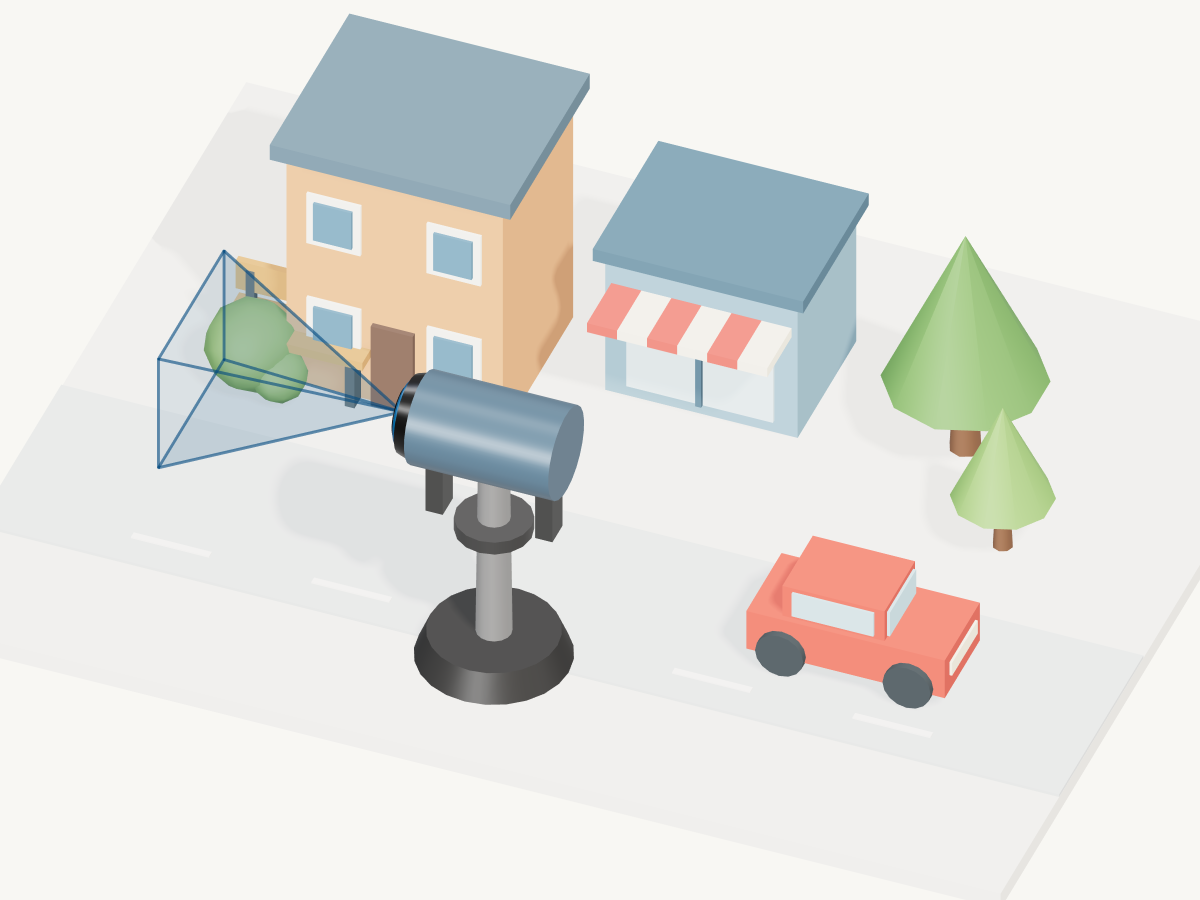
\includegraphics[width=6.6cm]{img/main/three/renders/two_scales_ptz.png}};

% Pan wraps beneath the camera base, clear of the background buildings.
\draw[actionarr, <->] ($(ptz.center)+(-1.43,-1.52)$)
  .. controls ($(ptz.center)+(-1.43,-2.0)$) and ($(ptz.center)+(0.27,-2.0)$)
  .. node[actionlabel, below] {pan} ($(ptz.center)+(0.27,-1.52)$);
% Tilt follows the camera head's height, beside its rear pivot.
\draw[actionarr, <->] ($(ptz.center)+(0.1,0.58)$)
  .. controls ($(ptz.center)+(0.57,0.43)$) and ($(ptz.center)+(0.57,-0.27)$)
  .. node[actionlabel, right] {tilt} ($(ptz.center)+(0.1,-0.42)$);
% Zoom runs parallel to the lens direction, below the viewing cone.
\draw[actionarr, <->] ($(ptz.center)+(-1.3,-0.62)$) -- node[actionlabel, below, sloped] {zoom} ($(ptz.center)+(-2.45,-0.3325)$);

\node[titletext, above=1.0cm of ptz] (lefttitle) {Local scale exploration};
\node[captiontext, below=0.15cm of lefttitle] (leftsubtitle) {where to look};
\node[captiontext, below=0.35cm of ptz] (leftcap) {fixed position, redirects gaze};

% ---------- right: global scale (UAV) ----------
\node[imgnode, right=2.6cm of ptz] (uav) {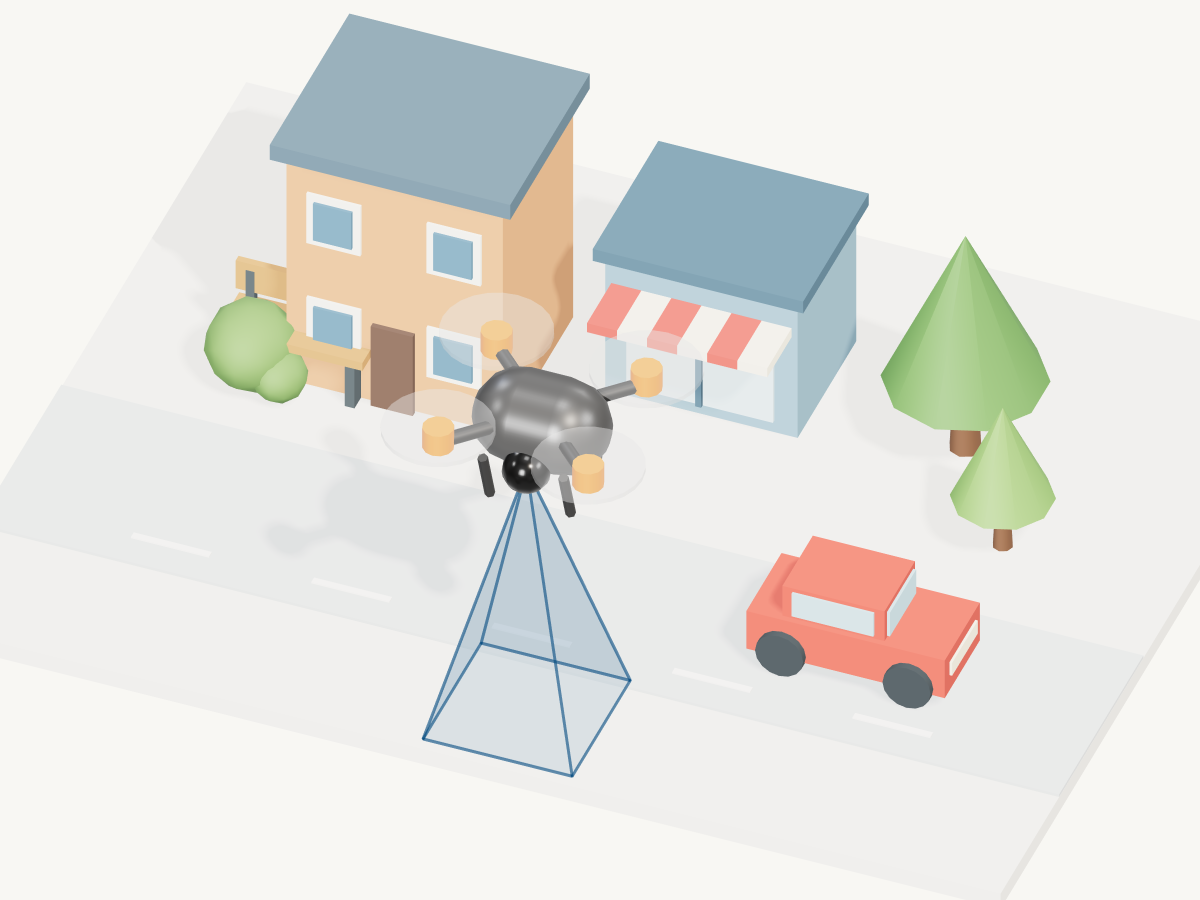
\includegraphics[width=6.6cm]{img/main/three/renders/two_scales_uav.png}};

% Place the shared origin in clear foreground to the left of the UAV.
% Steep ground-plane diagonals keep all three directions distinct.
% Opposite directions are dashed; z has exactly the same x at both ends.
\coordinate (axesorigin) at ($(uav.center)+(-1.65,-1.25)$);
\draw[actionarr, dashed] (axesorigin) -- ($(axesorigin)+(-0.63,0.51)$);
\draw[actionarr, dashed] (axesorigin) -- ($(axesorigin)+(0.675,0.35)$);
\draw[actionarr, dashed] (axesorigin) -- ($(axesorigin)+(0,-0.95)$);
\draw[actionarr] (axesorigin) -- node[actionlabel, left, pos=0.75] {z} ($(axesorigin)+(0,1.3)$);
\draw[actionarr] (axesorigin) -- node[actionlabel, below left, pos=0.7] {x} ($(axesorigin)+(1.05,-0.85)$);
\draw[actionarr] (axesorigin) -- node[actionlabel, below, pos=0.7] {y} ($(axesorigin)+(-1.35,-0.70)$);
\fill[steelblue31119180!70!black] (axesorigin) circle[radius=1.2pt];

\node[titletext, above=1.0cm of uav] (righttitle) {Global scale exploration};
\node[captiontext, below=0.15cm of righttitle] (rightsubtitle) {where to move};
\node[captiontext, below=0.35cm of uav] (rightcap) {physically relocates through 3D space};

% ---------- divider ----------
\node[fill=black!45, inner sep=0pt, minimum width=0.4pt, minimum height=8.6cm, anchor=north,
      right=1.3cm of ptz.east, yshift=0.55cm] {};

\end{tikzpicture}
